\documentclass{article}
\usepackage{graphicx} % Required for inserting images
\usepackage[hidelinks]{hyperref}
\usepackage{tablefootnote}
\usepackage{minted}
\usepackage{multicol}
\usepackage[sorting=none]{biblatex}
%\usepackage{fullpage}
\usepackage{comment}
\usepackage{tikz}
\usepackage{pgfplots}
\usepackage{booktabs}

\addbibresource{bib.bib}

\newcommand{\link}[1]{
\url{#1}
}
\newcommand{\linknourl}[1]{
\href{https://#1}{#1}
}

\title{\vspace{-2.5cm}Taming pthreads: Deterministic and\\Explorable Concurrency Fuzzing}
\author{Nathan Wachholz}
\date{June 17, 2023}

\begin{document}

\maketitle

\begin{abstract}
    \noindent We introduce a deterministic \texttt{pthread} implementation to assist fuzzing of concurrent software, and demonstrate its performance gains on a suite of benchmarks. We also investigate adding concurrency-coverage metrics to the \texttt{centipede} fuzzer, to further improve performance when fuzzing with our implementation.
\end{abstract}

\section{Introduction}

\sloppy
Fuzzing multi-threaded applications is tricky because scheduling is non-deterministic. Race conditions mean identical inputs can result in different executions and feature sets. However, efficiently fuzzing these applications is desirable, as many interesting targets are multi-threaded, and multi-threaded code is bug-prone.

\fussy

In this project, we introduce a deterministic \texttt{pthreads} implementation that is compatible with popular coverage-guided fuzzers. Specifically, our implementation\cite{my_unthread} ensures that identical inputs result in the same execution (assuming the rest of the program is deterministic). Furthermore, it allows a fuzzer to explore potential schedules with fine-grained control.

This enables the discovery of bugs that only occur under specific (potentially quite unlikely) thread schedules (see Appendix \ref{interleave} for an example). However, it also speeds up bug discovery in general, compared to running with a standard \texttt{pthreads} implementation. We evaluate our implementation on a suite of benchmarks, and show promising results.

Standard fuzzing feature-sets like code coverage can lead to schedule exploration, but there are a number of concurrency-coverage-metrics that directly incentivize it. We experiment with adding such metrics to the \texttt{centipede} fuzzer, making use of our \texttt{pthreads} implementation.

\subsection{Prior Work}

Concurrency is a well-studied problem in automated verification, and there are a variety of approaches. 

In the realm of symbolic execution and formal model checking, the \texttt{por-se}\cite{por-se} project is close to the state-of-the-art. It ``combines Partial-Order Reduction to detect interleaving non-determinism, with Symbolic Execution (SE) to handle data non-determinism.'' The project is an extension of KLEE (a popular symbolic executor), and can verify programs that use \texttt{pthreads}. Although POR techniques drastically reduce the search space of thread interleavings, program size is often a limiting factor. This is true of most static-analysis or symbolic-execution approaches--the search space of interleavings is gigantic.

Microsoft's CHESS\cite{chess} is a deterministic scheduler that exhaustively explores thread interleavings. It is usually run on an existing suite of unit tests, to ensure they pass regardless of thread schedule. CHESS has limits in debugging programs with missing or incomplete unit tests, and unit tests must remain somewhat small.

Applications that lack unit tests and are too large for symbolic execution are often fuzzed. On that front, Google's SockFuzzer\cite{sockfuzzer} is an effort to fuzz Apple's multi-threaded XNU kernel. It uses Concurrence\cite{concurrence}\cite{concurrence_presentation}, to run a single kernel thread at a time, with all scheduling decisions controlled by fuzzer input. This allows traditional fuzzing to continue deterministically, while also allowing the fuzzer to explore different schedules by mutating scheduling data. This is a very interesting technique, but it unfortunately remains quite specific to XNU, and cannot be used to fuzz arbitrary \texttt{pthread} applications.

\sloppy
Our goal with this project is to generalize SockFuzzer-like fuzzing to arbitrary \texttt{pthread} applications. In-process, coverage-guided fuzzing has a strong track-record of finding bugs, and we want to allow these fuzzers to effectively target \texttt{pthread} applications.

This brings us to \texttt{unthread}\cite{unthread}, a deterministic \texttt{pthreads} implementation. \texttt{unthread} has some notable shortcomings: not being completely POSIX-compliant; nor allowing schedule configuration at runtime. Nevertheless, it is a drop-in \texttt{pthreads} replacement that was a valuable starting point for this project. We extended \texttt{unthread} to work with \texttt{centipede} (a modern fuzzer), and performed experiments to show that fine-grained schedule control is beneficial. 

Academia and industry have turned to fuzzing for concurrency verification, and introduced various ``concurrency-coverage metrics'' to incentivize schedule exploration. This examined in more detail in Section \ref{section:metrics}, after we conclude our work with \texttt{unthread}.

\fussy

\section{Implementation}

It is critical that our implementation is as simple to use as possible. Ease-of-use makes can help tool adoption, but it also makes it easier for us to benchmark and test on a large suite of examples.

To this end, target code does not need to be modified. \texttt{unthread} ships an \texttt{pthread.h} header, and a single compiler flag can have it replace the builtin one. This header file redirects all \texttt{pthread\_XX} functions to \texttt{unthread\_XX} ones. All POSIX \texttt{pthread\_XX} functions are implemented, including synchronization primitives. Because all calls are intercepted, \texttt{unthread} can offer unique features such as deadlock detection: if all threads are blocked, the program will crash with a helpful error, rather than hanging.

\texttt{unthread} is implemented using user-space threads, frequently termed ``fibers''. These fibers run within a single host thread using \texttt{makecontext}, \texttt{swapcontext}, \texttt{setjmp}, and \texttt{longjmp}. At any moment, only one fiber is running. This means there is no preemption---context switches can only happen at specific ``yield points''. Almost any \texttt{pthread\_XX} call is a yield point (including the recommended \texttt{sched\_yield()}), which gives the scheduler the opportunity to switch to a different ``runnable'' thread.

A thread is runnable unless it is blocked (locking a mutex, joining another thread, etc.). At a yield point, the scheduler can switch to any runnable thread. If there is more than one runnable thread, then the scheduler has a ``scheduling decision''. The scheduler must pick one of the $n$ runnable threads to start executing. This is a deterministic decision, made according to a configurable ``data source''.

There are two possible data sources (also called ``scheduling control methods''), which are configured at runtime. The first is a stream of integers.  We consume an integer $k$ from the stream, and pick thread $k\,\%\,n$. The stream has a finite length, so the ``end behavior'' must also be defined. Options include looping, continuing with all zeros, terminating, etc.

The second option is a PRNG, which generates a stream of integers on the fly from a given ``seed''. Again, we generate an integer $k$, and pick thread $k\,\%\,n$. The PRNG is deterministic, depending only on the initial configured seed.

\sloppy

The user can configure \texttt{unthread} before each fuzzing input using the \texttt{unthread\_configure} call. This should be called from the fuzzing driver. For an example, see Appendix~\ref{appendix:driver}.

\fussy

Besides this call in the fuzzing driver and an additional compiler argument when building the target, there is no further user action required. Although not entirely compliant with POSIX (lack of preemption, fewer cancellation points, etc.), threading will become deterministic and reproducible. This is already any improvement over \texttt{pthreads}. In the next section, we will experimentally determine performance benefits.

\section{Evaluation and Results}

Although a deterministic \texttt{pthreads} implementation has other uses, the primary focus of this project is on fuzzing. Therefore, to evaluate performance, we will fuzz a suite of concurrent programs.

All programs in the suite take no input, but have a reachable bug (crash or deadlock), under some thread schedule. In theory, running any of these programs in a loop with \texttt{pthreads} will eventually result in a crash. We will check how the deterministic, explorable schedules provided by \texttt{unthread} can speed up this process.

We ran on a suite of 12 programs. They are described in Table~\ref{table:suite}. Most tests were adapted from existing sources, and information on each of those can be found through the SV-Comp project\cite{sv-comp}.

\begin{table}[ht]
  \centering
  \caption{Test Suite}
  \label{table:suite}
  \begin{tabular}{lll}
    \hline
    Test Name          & Source          & Category \\
    \hline
    \texttt{bigshot\_p}              & sv-comp         & mutex, trivial \\
    \texttt{bounded\_buffer}         & sv-comp         & mutex, trivial \\
    \texttt{checkpoints}    & -          & very rare schedule \\
    \texttt{deadlock\_1}             & sctbench        & deadlock \\
    \texttt{interleave}     & -          & very rare schedule \\
    \texttt{lazy}           & sv-benchmarks   & rare schedule \\
    \texttt{phase\_1}                & sctbench        & deadlock \\
    \texttt{singleton\_b}   & sv-benchmarks   & very rare schedule \\
    \texttt{stringbuffer}   & Jie Yu\tablefootnote{Mimics a concurrency bug in JDK1.4 StringBuffer, by Jie Yu (jieyu@umich.edu)}          & rare schedule, mutex \\
    \texttt{triangular}     & sv-benchmarks   & very rare schedule \\
    \texttt{workstealqueue\_mutex\_1} & sv-comp         & mutex \\
    \texttt{workstealqueue\_mutex\_3} & sv-comp         & mutex \\
    \hline
  \end{tabular}
\end{table}

Tests were performed using the Centipede\cite{centipede} fuzzer. For comparison, we fuzzed each program in one of three ways. (1) Using the standard \texttt{pthread} implementation; (2) With the fuzzer varying \texttt{unthread}'s PRNG seed; and (3) With the fuzzer varying \texttt{unthread}'s schedule data.

\subsection{Results}

Each fuzzer-target-pair, was given 15 minutes to run as many times as possible. A run ends when a bug (crash or deadlock) is found. In the case of pthread, there is no deadlock detection, so we rely on a 10 second timeout per input. We record the average time-to-bug of each pair, which is presented in Table~\ref{table:results}. If the fuzz-target-pair doesn't find a bug within 15 minutes, we record ``timeout''. The inverse of these times (a measure of speed) is illustrated in Figure~\ref{fig:results}.

\begin{figure}[h]
    \centering

    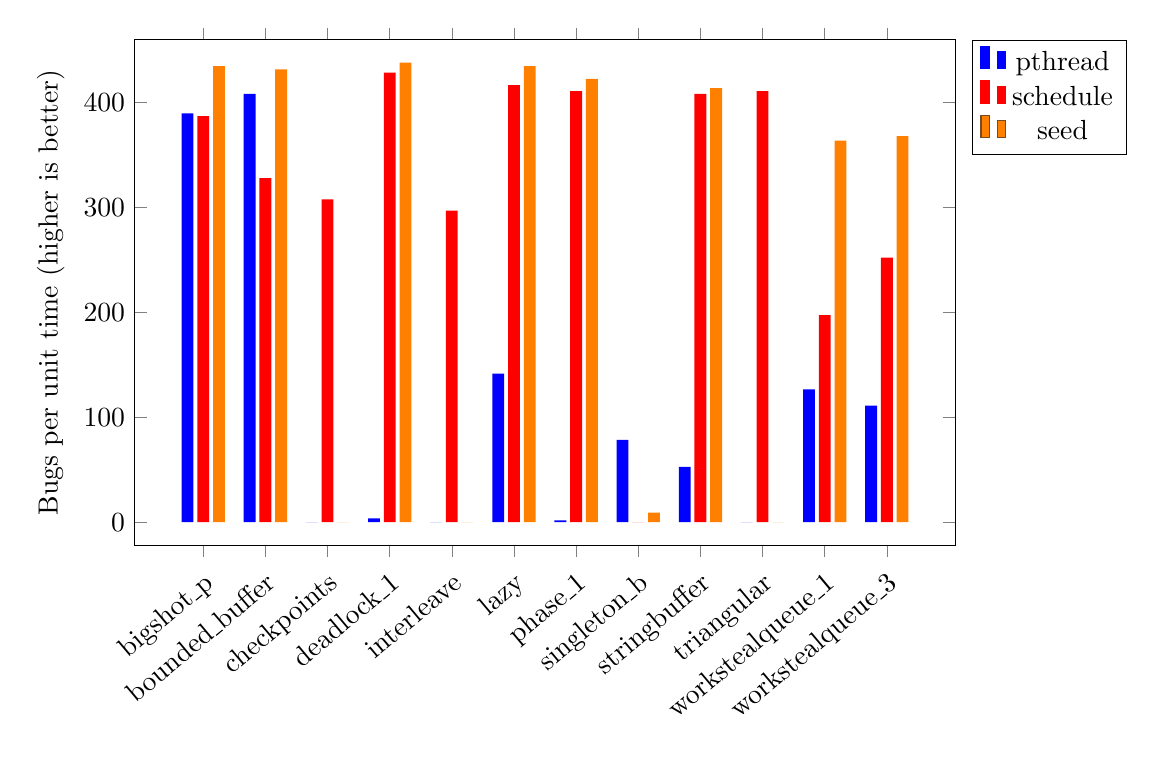
\begin{tikzpicture}
    \begin{axis}[
    	x tick label style={
    		/pgf/number format/1000 sep=},
    	ylabel=Bugs per unit time (higher is better),
    	enlargelimits=0.05,
     xtick=data,
    xticklabels={bigshot\_p, bounded\_buffer, checkpoints, deadlock\_1, interleave, lazy, phase\_1, singleton\_b, stringbuffer, triangular, workstealqueue\_1, workstealqueue\_3},
    xticklabel style={rotate=40, anchor=north east},
    enlarge x limits={0.1},
    width=12cm,
    height=8cm,
    legend style={at={(1.02,1)}, anchor=north west, legend columns=1},
    bar width=0.15cm,
    ybar=-0.6cm, 
]

\addplot+[bar shift=-0.2cm, fill=blue, draw=none] coordinates {(1, 389.610) (2, 408.163) (3, 0.000) (4, 3.542) (5, 0.000) (6, 141.509) (7, 1.810) (8, 78.431) (9, 52.724) (10, 0.000) (11, 126.582) (12, 111.111)};
\addplot+[bar shift=0cm, fill=red, draw=none] coordinates {(1, 387.097) (2, 327.869) (3, 307.692) (4, 428.571) (5, 297.030) (6, 416.667) (7, 410.959) (8, 0.000) (9, 408.163) (10, 410.959) (11, 197.368) (12, 252.101)};
\addplot+[bar shift=0.2cm, fill=orange, draw=none] coordinates {(1, 434.783) (2, 431.655) (3, 0.000) (4, 437.956) (5, 0.000) (6, 434.783) (7, 422.535) (8, 8.993) (9, 413.793) (10, 0.000) (11, 363.636) (12, 368.098)};

\legend{pthread, schedule, seed}

    \end{axis}
    \end{tikzpicture}
    
    \caption{A comparison of fuzzing speed on a variety of targets using three scheduling control methods.}
    \label{fig:results}
\end{figure}

\begin{table}[h]
  \centering
  \begin{tabular}{lrrr}
    \toprule
    Name & pthread & schedule & seed \\
    \midrule
    \texttt{bigshot\_p}                & 0.154   & 0.155   & 0.138 \\
    \texttt{bounded\_buffer}           & 0.147   & 0.183   & 0.139 \\
    \texttt{checkpoints}               & timeout & 0.195   & timeout \\
    \texttt{deadlock\_1}               & 16.940 & 0.140   & 0.137 \\
    \texttt{interleave}                & timeout & 0.202   & timeout \\
    \texttt{lazy}                      & 0.424   & 0.144   & 0.138 \\
    \texttt{phase\_1}                  & 33.149 & 0.146   & 0.142 \\
    \texttt{singleton\_b}              & 0.765   & timeout & 6.672 \\
    \texttt{stringbuffer}              & 1.138  & 0.147   & 0.145 \\
    \texttt{triangular}                & timeout & 0.146   & timeout \\
    \texttt{workstealqueue\_mutex\_1}  & 0.474   & 0.304   & 0.165 \\
    \texttt{workstealqueue\_mutex\_3}  & 0.540   & 0.238   & 0.163 \\
    \bottomrule
  \end{tabular}
  \caption{Average Fuzzing Time-to-bug (seconds)}
  \label{table:results}
\end{table}

These results align with our expectations (with some exceptions). First of all, the two deadlock tests (\texttt{deadlock\_1} and \texttt{phase\_1}) competed much faster with \texttt{unthread}, due to its deadlock-reporting capabilities. Of course, the exact performance difference depends on the configured test timeout (we used 10 seconds, the default is 60). 

Second, we expect \texttt{unthread} to outperform \texttt{pthread} in all but the most simple tests (\texttt{bigshot\_p}, \texttt{bounded\_buffer}). While this is generally true, the exact speedup varies. In some cases, \texttt{pthread} could not find the bug within 15 minutes, whereas \texttt{unthread} found it in under a second (\texttt{interleave}, \texttt{checkpoints}, \texttt{triangular}). 

Lastly, we expected schedule data to outperform PRNG seed. This is not so clear-cut. Generally, seed was faster than schedule, unless the schedule required was exceedingly rare (\texttt{interleave}, \texttt{checkpoints}, \texttt{triangular}) and seed couldn't get it at all.

There was one unusual result with the \texttt{singleton\_b} example. This case creates 11 threads. Each thread sets a constant to \texttt{'Y'} except one, which sets it to \texttt{'X'}. The X thread must run last for the crash to occur. It's unclear why \texttt{pthread} excels in this case, but it is clear why \texttt{unthread} struggles: there are no features to distinguish different schedules. In the following section, we discuss our attempts to add ``concurrency coverage metrics'' to solve this problem.

\section{Concurrency Coverage Metrics}\label{section:metrics}

At this point, we have succeeded in creating a \texttt{pthread} implementation to speed up fuzzing of concurrent programs with a deterministic schedule. However, the fuzzer has no direct measure of ``concurrency coverage''. Even if two test inputs result in a different interleaving order, the actual lines of code executed (and the resulting fuzzing features) may be the same. There is no incentive for the fuzzer to try different interleavings, unless it gets lucky and they result in different features.

\sloppy

This is a well studied problem, and there have been a few proposed ``concurrency-coverage metrics''. \cite{cfp} proposes Concurrent Function Pairs (CFP), which count how often each pair of functions are executed in parallel. Another is Concurrent Basic Block Pairs, which is the same but for basic blocks. And recently, Concurrent Context Pairs\cite{ccp} (CCP), which is like CFP but includes a few more levels of the call stack.

We attempt to implement something similar to CCP. Each thread $T$ maintains a hash of its call stack ($callstack(T)$, using an array of PCs from \texttt{\_\_builtin\_return\_address(level)}). The depth of the callstack is configurable.

\fussy

At each context switch, we record a features. When switching from thread $S$ to thread $T$, we record a hash of the tuple $(callstack(S), callstack(T))$.

Centipede makes user-defined features easy. \texttt{unthread} declares an array in the special \texttt{section("\_\_centipede\_extra\_features")}, and populates the array with integers corresponding to each custom feature.

Unfortunately, after implementing the custom features, there was little to no affect on performance. While the fuzzer was recording and reporting the new features for each input, the number of features was much higher than expected, and they would change between runs (so they were not deterministic). After more investigating, we realized some issues with our approach. Although we did not have time to address them, they are outlined in the Section~\ref{section:metrics-challenges}.

\section{Challenges}

In this section, we describe challenges encountered during this project. We hope this explains our design decisions, and gives ideas for future work or improvements.

\subsection{Integrating \texttt{unthread}}

Initially, \texttt{unthread} used the same symbol names as \texttt{pthreads}. This made switching between implementations easy. No code needed to be modified. However, because \texttt{unthread} uses different, simpler types and structures, recompilation was still required. Recompilation only required using a different \texttt{pthread.h} header, which could be done with an additional compiler argument.

However, we quickly ran into issues with this approach. The C++ standard library uses \texttt{pthread} calls, and was not compiled with our header. This caused crashes very early in program startup. 

Our next approach was similar. Each thread would maintain a thread-local variable denoting if the thread was from \texttt{pthread} or \texttt{unthread}. \texttt{unthread} would continue to use \texttt{pthread} symbol names, but would optionally forward the call to \texttt{pthreads} using \texttt{dlsym}, based on the thread-local variable. There was a function to switch a thread to using \texttt{unthread}, which would be called by the fuzzing driver prior to executing the target. 

This worked well for simple targets. However, we quickly realized that instrumented code uses \texttt{pthreads} (such as ASAN). We want to redirect the instrumentation to \texttt{pthreads}, because that's how it was initialized, but we could easily determine where calls were coming from. The edge cases and complexity of this solution was too much, and we reevaluated again.

We finally settled on the current approach. Since recompiling with a different header is already required, we simply \texttt{\#define} each \texttt{pthread\_XX} function to the corresponding \texttt{unthread\_XX} one. This works well.

\subsection{Memory Leak}

After connecting \texttt{unthread} to our fuzzing harness for the first time, we would get an out-of-memory crash within a few hundred executions of the fuzzer. Some debugging uncovered a bug in \texttt{unthread}'s memory management, causing it to never free a thread's stack space. The fix was fairly simple, and was merged back into \texttt{unthread} via PR \#4\cite{unthread_pr}.

\subsection{Concurrency Coverage Metrics}\label{section:metrics-challenges}

As mentioned in Section~\ref{section:metrics}, we attempted to add concurrency-coverage metrics to centipede. Unfortunately, we experienced a blowup of features, and non-determinism between runs. 

\sloppy 

Our hashes and features are determined by walking up the call stack and recording the PC as reported by \texttt{\_\_builtin\_return\_address(level)} and \texttt{\_\_builtin\_extract\_return\_addr}. Unfortunately, this doesn't account for PIE. The same function will be loaded into a different place for each run. This means that the hashes will be completely different each time, explaining our results.

\fussy

There was no solution to this issue we could implement within the time allotted. Theoretically, we could use \texttt{dladdr} to determine the object base address. Then all addresses could be hashed relative to their object's base address. This would undoubtedly get slow, so we would likely need to add a cache.

Another option is to reuse \texttt{centipede}'s existing thread stack features, modifying them to work with \texttt{unthread}. This might be cleaner, but would necessitate a closer integration between the two projects.

\section{Conclusion}

\sloppy

This project introduced an ready-to-use solution to improve concurrency fuzzing. Our technique can quickly find bugs that can't be found otherwise. It is able to instantly detect deadlocks--and can describe the deadlock to help with debugging. We showed promising results, demonstrating sizeable speedups on 10 of 12 benchmarks. Although concurrency-coverage metrics aren't working, we believe they could with a little more effort.

There's a lot of potential here, and a few promising next steps:

\begin{itemize}
    \item Use \texttt{unthread} with more realistic targets, such as adding it to OSS-Fuzz\cite{oss-fuzz}.
    \item Fix concurrency-coverage metrics to overcome PIE.
    \item Closer integration with centipede (or other fuzzers). For instance, separating schedule data from the rest of the fuzzing input.
\end{itemize}

\newpage

\nocite{*}
\printbibliography

\section{Appendix}

\subsection{Interleave Example} \label{interleave}

Here is the \texttt{interleave} example from our benchmark suite. It illustrates an extreme example of the kind of bug we would like to detect. Although contrived, the following program has a bug that is only reachable under a \textit{very} specific schedule: 

\begin{multicols}{2}
\begin{minted}{c}
void* buggy(int *val) {
  // buggy must be the first 
  // to execute
  if(*val != 0) return 0; 
  pthread_yield();
  // incr must execute 2 times,
  // then back to buggy
  if(*val != 2) return 0; 
  pthread_yield();
  // incr must execute 3 times, 
  // then back to buggy
  if(*val != 5) return 0;
  pthread_yield();
  // etc.
  if(*val != 7) return 0;
  pthread_yield();

  if(*val != 12) return 0;
  pthread_yield();

  if(*val != 15) return 0;
  pthread_yield();

  if(*val == 17) {
    __builtin_trap(); // a "bug"!
  }
}
\end{minted}
\columnbreak
\begin{minted}{c}
void* incr(int* val) {
  while(*val < 20) {
    pthread_yield();
    (*val)++;
  }
}

void interleave() {
  int val = 0;
  
  pthread_t a, b;
  pthread_create(&a, NULL, 
                 incr, &val);
  pthread_create(&b, NULL, 
                 buggy, &val);
  pthread_join(a, NULL);
  pthread_join(b, NULL);
}

int main() {
  interleave();
}
\end{minted}
\end{multicols}

Specifically, to reach the ``bug'', the scheduler needs to make the correct choice of thread to resume at each of at least 25 yield points\footnote{at least 2 in \texttt{main} during thread creation, 6 in \texttt{buggy}, 17 in \texttt{incr}}. It's reasonable to say that a random schedule has a probability of \textit{at best} 1 in $2^{25}$ $(1/33,554,432)$ to trigger the bug.

Using \texttt{centipede} and \texttt{unthread}, the bug is reached in 0.1s. After running with \texttt{pthreads} for 5 days, it still hadn't found the bug. In a real target, the ``bug'' could be from a sanitizer (ASAN, MSAN, TSAN, etc.), an assertion failure, or any other crash.

\subsection{Fuzzing Drivers} \label{appendix:driver}

Here is an example of our fuzzing drivers, and demonstrating how to configure \texttt{unthread}.

\begin{minted}{C}
int LLVMFuzzerTestOneInput(const uint8_t *data, size_t size) {
  // Schedule data
  unthread_configure((struct entropy_configuration){
    .entropy_source = ENTROPY_SCHEDULE,
    .schedule = {
      .data = (uint32_t*) data,
      .data_len = size / sizeof(uint32_t),
      .end_behavior = SCHEDULE_END_ZEROS,
    },
  });
  
  interleave();
}

int LLVMFuzzerTestOneInput(const uint8_t *data, size_t size) {
  // PRNG Seed
  uint32_t state[4] = {0, 0, 0, 0};
  if(size > sizeof(state)) {
    return 0;
  }
  memcpy((void *) state, data, size);
  
  unthread_configure((struct entropy_configuration){
    .entropy_source = ENTROPY_PRNG_SEED,
    .prng_seed = {
      .state = {state[0], state[1], state[2], state[3]},
    },
  });
  
  interleave();
}
\end{minted}

\end{document}
